\documentclass{article}

\usepackage{../../noweb}
\noweboptions{smallcode,longchunks}

\usepackage[a4paper,margin=1in]{geometry}

\usepackage{colortbl}
\usepackage[colorlinks=true]{hyperref}
\usepackage{graphicx}

% Remove noweb page break penalty
\def\nwendcode{\endtrivlist \endgroup}
\let\nwdocspar=\par

\title{Jargo Storage Interface
  and Data Model\footnote{\url{https://github.com/jargors/Storage}}\\
  \vspace{.5em}
  \Large{\textbf{Performance Test Program}}}
\author{James J. Pan\\
  \small{\href{mailto:jamesjpan@outlook.com}{jamesjpan@outlook.com}}
}

\begin{document}
\maketitle
\pagestyle{noweb}

%\begin{figure}[h]
%\centering
%\fbox{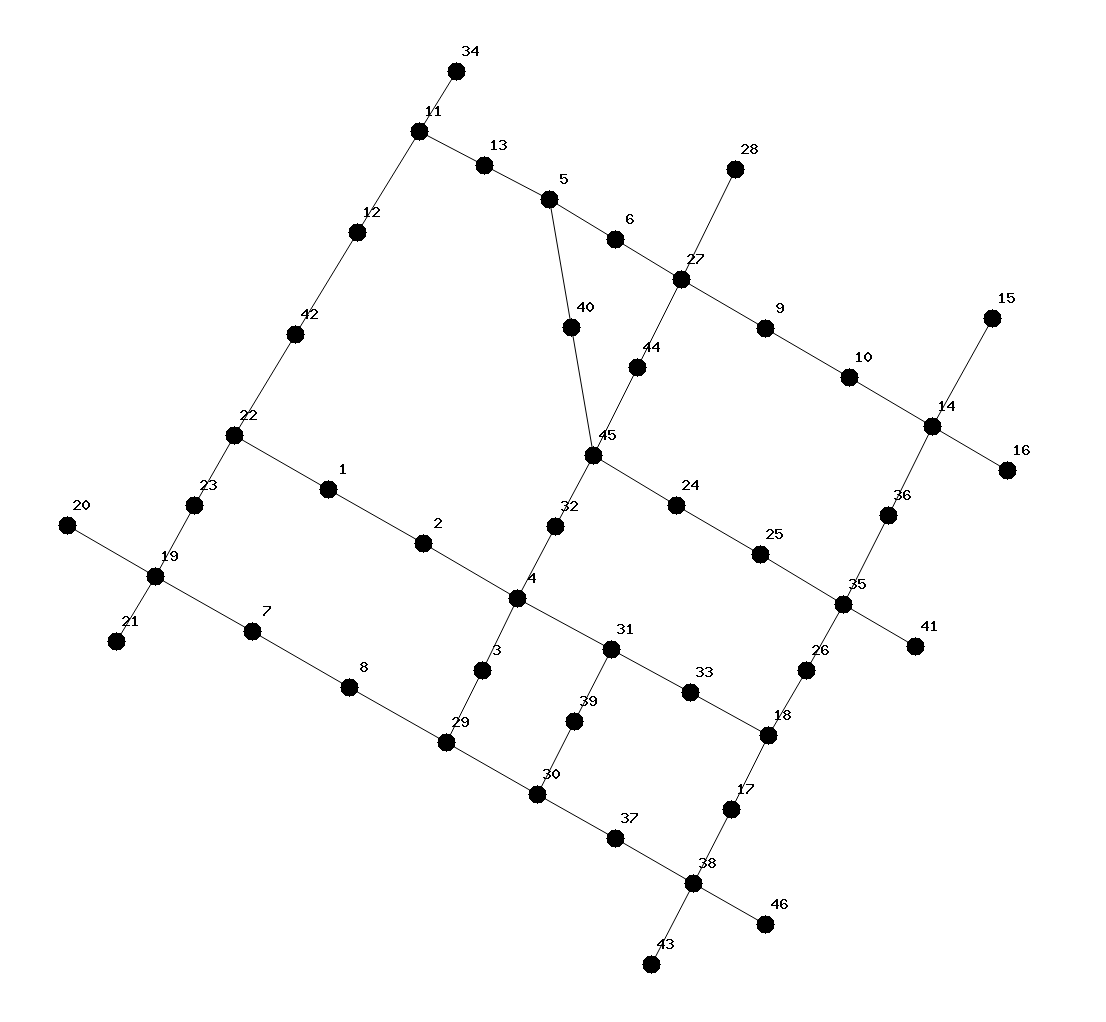
\includegraphics[width=\textwidth]{data/test.png}}
%\caption{Portion of a road network in Chengdu, China,
%    used for tests (46 nodes, 104 directed edges).}
%\label{fig:road-network}
%\end{figure}
%\newpage

\tableofcontents

\section{Introduction}
\label{sec:introduction}
The test program is developed using the
Noweb\footnote{\url{https://www.cs.tufts.edu/~nr/noweb/}} literate
programming\footnote{\url{http://literateprogramming.com/}} tool.  This file
({\tt{}src/StoragePerformanceTest.nw}) is the source for both the documentation
({\tt{}doc/StoragePerformanceTest.tex}) and the Java code
({\tt{}StoragePerformanceTest.java})\footnote{See the {\tt{}Makefile} for build
details.}.
\nwfilename{src/StoragePerformanceTest.nw}\nwbegincode{1}\sublabel{NW3iKWou-40YM6y-1}\nwmargintag{{\nwtagstyle{}\subpageref{NW3iKWou-40YM6y-1}}}\moddef{StoragePerformanceTest.java~{\nwtagstyle{}\subpageref{NW3iKWou-40YM6y-1}}}\endmoddef\nwnotused{StoragePerformanceTest.java}
\LA{}StoragePerformanceTest.java preamble~{\nwtagstyle{}\subpageref{NW3iKWou-2PlaJO-1}}\RA{}
\LA{}\code{}StoragePerformanceTest\edoc{} definition~{\nwtagstyle{}\subpageref{NW3iKWou-490CRJ-1}}\RA{}
\nwendcode{}\nwbegindocs{2}\nwdocspar

\nwenddocs{}\nwbegincode{3}\sublabel{NW3iKWou-2PlaJO-1}\nwmargintag{{\nwtagstyle{}\subpageref{NW3iKWou-2PlaJO-1}}}\moddef{StoragePerformanceTest.java preamble~{\nwtagstyle{}\subpageref{NW3iKWou-2PlaJO-1}}}\endmoddef\nwused{\\{NW3iKWou-40YM6y-1}}
import com.github.jargors.Controller;
import com.github.jargors.Storage;
import com.github.jargors.Tools;
import com.github.jargors.exceptions.DuplicateVertexException;
import com.github.jargors.exceptions.DuplicateEdgeException;
import com.github.jargors.exceptions.DuplicateUserException;
import com.github.jargors.exceptions.EdgeNotFoundException;
import com.github.jargors.exceptions.UserNotFoundException;
import com.github.jargors.exceptions.VertexNotFoundException;
import java.time.LocalDateTime;
import java.sql.Connection;
import java.sql.Statement;
import java.sql.SQLException;
\nwendcode{}\nwbegindocs{4}\nwdocspar

\nwenddocs{}\nwbegincode{5}\sublabel{NW3iKWou-490CRJ-1}\nwmargintag{{\nwtagstyle{}\subpageref{NW3iKWou-490CRJ-1}}}\moddef{\code{}StoragePerformanceTest\edoc{} definition~{\nwtagstyle{}\subpageref{NW3iKWou-490CRJ-1}}}\endmoddef\nwused{\\{NW3iKWou-40YM6y-1}}
public class StoragePerformanceTest \{
  \LA{}\code{}StoragePerformanceTest\edoc{} member variables~{\nwtagstyle{}\subpageref{NW3iKWou-5sgeP-1}}\RA{}
  \LA{}\code{}StoragePerformanceTest\edoc{} main routine~{\nwtagstyle{}\subpageref{NW3iKWou-2hjWc8-1}}\RA{}
  \LA{}\code{}StoragePerformanceTest\edoc{} private methods~{\nwtagstyle{}\subpageref{NW3iKWou-1GKv5n-1}}\RA{}
\}
\nwendcode{}\nwbegindocs{6}\nwdocspar
\nwenddocs{}\nwbegincode{7}\sublabel{NW3iKWou-5sgeP-1}\nwmargintag{{\nwtagstyle{}\subpageref{NW3iKWou-5sgeP-1}}}\moddef{\code{}StoragePerformanceTest\edoc{} member variables~{\nwtagstyle{}\subpageref{NW3iKWou-5sgeP-1}}}\endmoddef\nwused{\\{NW3iKWou-490CRJ-1}}
\nwendcode{}\nwbegindocs{8}%def

\nwenddocs{}\nwbegincode{9}\sublabel{NW3iKWou-2hjWc8-1}\nwmargintag{{\nwtagstyle{}\subpageref{NW3iKWou-2hjWc8-1}}}\moddef{\code{}StoragePerformanceTest\edoc{} main routine~{\nwtagstyle{}\subpageref{NW3iKWou-2hjWc8-1}}}\endmoddef\nwused{\\{NW3iKWou-490CRJ-1}}
public static void main(String[] args) \{
  Print("Starting storage performance tests");
  try \{
    \LA{}Load performance tests~{\nwtagstyle{}\subpageref{NW3iKWou-xbUR1-1}}\RA{}
  \} catch (SQLException e) \{
    Tools.PrintSQLException(e);
  \}
  Print("Complete!");
\}
\nosublabel{NW3iKWou-2hjWc8-1-u1}\nwindexdefn{main}{main}{NW3iKWou-2hjWc8-1}\eatline
\nwidentdefs{\\{{main}{main}}}\nwendcode{}\nwbegindocs{10}\nwdocspar
\nwenddocs{}\nwbegincode{11}\sublabel{NW3iKWou-4SyIkm-1}\nwmargintag{{\nwtagstyle{}\subpageref{NW3iKWou-4SyIkm-1}}}\moddef{Begin timing block~{\nwtagstyle{}\subpageref{NW3iKWou-4SyIkm-1}}}\endmoddef\nwused{\\{NW3iKWou-3EFvya-1}\\{NW3iKWou-39EpqO-1}\\{NW3iKWou-3kKW1I-1}\\{NW3iKWou-29RW2s-1}}
long _t0 = System.currentTimeMillis();
int _count = 0;
float _dur = 0;
\nwendcode{}\nwbegindocs{12}\nwdocspar

\nwenddocs{}\nwbegincode{13}\sublabel{NW3iKWou-3FrbVy-1}\nwmargintag{{\nwtagstyle{}\subpageref{NW3iKWou-3FrbVy-1}}}\moddef{Increment call count~{\nwtagstyle{}\subpageref{NW3iKWou-3FrbVy-1}}}\endmoddef\nwused{\\{NW3iKWou-3EFvya-1}\\{NW3iKWou-39EpqO-1}\\{NW3iKWou-3kKW1I-1}\\{NW3iKWou-29RW2s-1}}
System.out.print("\\r          \\r"+_count);
_count++;
\nwendcode{}\nwbegindocs{14}\nwdocspar

\nwenddocs{}\nwbegincode{15}\sublabel{NW3iKWou-3FOZIi-1}\nwmargintag{{\nwtagstyle{}\subpageref{NW3iKWou-3FOZIi-1}}}\moddef{End timing block~{\nwtagstyle{}\subpageref{NW3iKWou-3FOZIi-1}}}\endmoddef\nwused{\\{NW3iKWou-3EFvya-1}\\{NW3iKWou-39EpqO-1}\\{NW3iKWou-3kKW1I-1}\\{NW3iKWou-29RW2s-1}}
long _t1 = System.currentTimeMillis();
_dur=((_t1 - _t0)/(float)(_count == 0 ? 1 : _count));
System.out.print("\\r");
\nwendcode{}\nwbegindocs{16}\nwdocspar

Until I figure out how to close the Derby DB after each test, these
can only be performed one at a time.
\nwenddocs{}\nwbegincode{17}\sublabel{NW3iKWou-xbUR1-1}\nwmargintag{{\nwtagstyle{}\subpageref{NW3iKWou-xbUR1-1}}}\moddef{Load performance tests~{\nwtagstyle{}\subpageref{NW3iKWou-xbUR1-1}}}\endmoddef\nwused{\\{NW3iKWou-2hjWc8-1}}
/*\LA{}Test \code{}{\char95}getConnection\edoc{}(0)~{\nwtagstyle{}\subpageref{NW3iKWou-3EFvya-1}}\RA{}*/
/*\LA{}Test \code{}DBAddNewServer\edoc{}(1)~{\nwtagstyle{}\subpageref{NW3iKWou-39EpqO-1}}\RA{}*/
/*\LA{}Test \code{}DBQueryQueuedRequests\edoc{}(1)~{\nwtagstyle{}\subpageref{NW3iKWou-3kKW1I-1}}\RA{}*/
\LA{}Test \code{}DBQueryServerLocationsActive\edoc{}(1)~{\nwtagstyle{}\subpageref{NW3iKWou-29RW2s-1}}\RA{}
\nwendcode{}\nwbegindocs{18}\nwdocspar

\nwenddocs{}\nwbegincode{19}\sublabel{NW3iKWou-3EFvya-1}\nwmargintag{{\nwtagstyle{}\subpageref{NW3iKWou-3EFvya-1}}}\moddef{Test \code{}{\char95}getConnection\edoc{}(0)~{\nwtagstyle{}\subpageref{NW3iKWou-3EFvya-1}}}\endmoddef\nwused{\\{NW3iKWou-xbUR1-1}}
\{
  Storage storage = new Storage();
  final int n = 10000;  // 10,000
  Connection[] arr = new Connection[n];
  \LA{}Begin timing block~{\nwtagstyle{}\subpageref{NW3iKWou-4SyIkm-1}}\RA{}
  for (int i = 0; i < n; i++) \{
    arr[i] = storage._getConnection();
    \LA{}Increment call count~{\nwtagstyle{}\subpageref{NW3iKWou-3FrbVy-1}}\RA{}
  \}
  \LA{}End timing block~{\nwtagstyle{}\subpageref{NW3iKWou-3FOZIi-1}}\RA{}
  Print("_getConnection(0): "+_dur+" ms/call");
  for (Connection c : arr) \{
    try \{
      c.close();
    \} catch (Exception e) \{ \}
  \}
\}
\nwendcode{}\nwbegindocs{20}\nwdocspar

\nwenddocs{}\nwbegincode{21}\sublabel{NW3iKWou-39EpqO-1}\nwmargintag{{\nwtagstyle{}\subpageref{NW3iKWou-39EpqO-1}}}\moddef{Test \code{}DBAddNewServer\edoc{}(1)~{\nwtagstyle{}\subpageref{NW3iKWou-39EpqO-1}}}\endmoddef\nwused{\\{NW3iKWou-xbUR1-1}}
\{
  Controller controller = new Controller();
  controller.loadDataModel();
  controller.loadRoadNetwork("data/chengdu.rnet");
  controller.loadGTree("data/chengdu.gtree");
  final int n = 1000;  // 1,000
  \LA{}Begin timing block~{\nwtagstyle{}\subpageref{NW3iKWou-4SyIkm-1}}\RA{}
  for (int i = 0; i < n; i++) \{
    int o = (int) Math.round(Math.random()*32934);
    int d = (int) Math.round(Math.random()*32934);
    controller.addNewServer(new int[] \{ i, -1, 0, 86400000, o, d, 1 \});
    \LA{}Increment call count~{\nwtagstyle{}\subpageref{NW3iKWou-3FrbVy-1}}\RA{}
  \}
  \LA{}End timing block~{\nwtagstyle{}\subpageref{NW3iKWou-3FOZIi-1}}\RA{}
  Print("DBAddNewServer(1): "+_dur+" ms/call");
\}
\nwendcode{}\nwbegindocs{22}\nwdocspar

Even though {\tt{}Controller} falls out of scope from the previous test,
the Derby database is still live! No need to load data model, road network
again.
\nwenddocs{}\nwbegincode{23}\sublabel{NW3iKWou-3kKW1I-1}\nwmargintag{{\nwtagstyle{}\subpageref{NW3iKWou-3kKW1I-1}}}\moddef{Test \code{}DBQueryQueuedRequests\edoc{}(1)~{\nwtagstyle{}\subpageref{NW3iKWou-3kKW1I-1}}}\endmoddef\nwused{\\{NW3iKWou-xbUR1-1}}
\{
  Controller controller = new Controller();
  controller.loadDataModel();
  controller.loadRoadNetwork("data/chengdu.rnet");
  controller.loadGTree("data/chengdu.gtree");
  controller.loadProblem("data/chengdu.instance");
  int[] output = new int[] \{ \};
  \LA{}Begin timing block~{\nwtagstyle{}\subpageref{NW3iKWou-4SyIkm-1}}\RA{}
  for (int t = 0; t < 1800; t++) \{
    output = controller.queryQueuedRequests(t);
    \LA{}Increment call count~{\nwtagstyle{}\subpageref{NW3iKWou-3FrbVy-1}}\RA{}
  \}
  \LA{}End timing block~{\nwtagstyle{}\subpageref{NW3iKWou-3FOZIi-1}}\RA{}
  Print("DBQueryQueuedRequests(1): "+_dur+" ms/call");
\}
\nwendcode{}\nwbegindocs{24}\nwdocspar

\nwenddocs{}\nwbegincode{25}\sublabel{NW3iKWou-29RW2s-1}\nwmargintag{{\nwtagstyle{}\subpageref{NW3iKWou-29RW2s-1}}}\moddef{Test \code{}DBQueryServerLocationsActive\edoc{}(1)~{\nwtagstyle{}\subpageref{NW3iKWou-29RW2s-1}}}\endmoddef\nwused{\\{NW3iKWou-xbUR1-1}}
\{
  Storage storage = new Storage();
  storage.DBLoadBackup("data/db");
  storage.DBLoadRoadNetworkFromDB();
  storage.DBLoadUsersFromDB();
  // BACKUP DOS NOT HAVE INDEXES
  try \{
    Connection conn = storage._getConnection();
    Statement stmt = conn.createStatement();
    stmt.addBatch("CREATE INDEX W_sid_t1 ON W (sid, t1)");
    stmt.addBatch("CREATE INDEX W_sid_t2 ON W (sid, t2)");
    stmt.addBatch("CREATE INDEX W_sid_v2 ON W (sid, v2)");
    stmt.addBatch("CREATE INDEX W_sid_t1_t2 ON W (sid, t1, t2)");
    stmt.executeBatch();
    conn.commit();
    conn.close();
  \} catch (Exception e) \{
    Print(e.toString());
  \}
  int[] output = new int[] \{ \};
  \LA{}Begin timing block~{\nwtagstyle{}\subpageref{NW3iKWou-4SyIkm-1}}\RA{}
  for (int t = 0; t < 1800; t+=100) \{
    output = storage.DBQueryServerLocationsActive(t);
    \LA{}Increment call count~{\nwtagstyle{}\subpageref{NW3iKWou-3FrbVy-1}}\RA{}
  \}
  \LA{}End timing block~{\nwtagstyle{}\subpageref{NW3iKWou-3FOZIi-1}}\RA{}
  Print("DBQueryServerLocationsActive(1): "+_dur+" ms/call");
\}
\nwendcode{}\nwbegindocs{26}\nwdocspar

\nwenddocs{}\nwbegincode{27}\sublabel{NW3iKWou-1GKv5n-1}\nwmargintag{{\nwtagstyle{}\subpageref{NW3iKWou-1GKv5n-1}}}\moddef{\code{}StoragePerformanceTest\edoc{} private methods~{\nwtagstyle{}\subpageref{NW3iKWou-1GKv5n-1}}}\endmoddef\nwused{\\{NW3iKWou-490CRJ-1}}
private static void Print(String msg) \{
  System.out.println("[StoragePerformanceTest]["+LocalDateTime.now()+"] "+msg);
\}
\nwendcode{}

\nwixlogsorted{c}{{\code{}StoragePerformanceTest\edoc{} definition}{NW3iKWou-490CRJ-1}{\nwixu{NW3iKWou-40YM6y-1}\nwixd{NW3iKWou-490CRJ-1}}}%
\nwixlogsorted{c}{{\code{}StoragePerformanceTest\edoc{} main routine}{NW3iKWou-2hjWc8-1}{\nwixu{NW3iKWou-490CRJ-1}\nwixd{NW3iKWou-2hjWc8-1}}}%
\nwixlogsorted{c}{{\code{}StoragePerformanceTest\edoc{} member variables}{NW3iKWou-5sgeP-1}{\nwixu{NW3iKWou-490CRJ-1}\nwixd{NW3iKWou-5sgeP-1}}}%
\nwixlogsorted{c}{{\code{}StoragePerformanceTest\edoc{} private methods}{NW3iKWou-1GKv5n-1}{\nwixu{NW3iKWou-490CRJ-1}\nwixd{NW3iKWou-1GKv5n-1}}}%
\nwixlogsorted{c}{{Begin timing block}{NW3iKWou-4SyIkm-1}{\nwixd{NW3iKWou-4SyIkm-1}\nwixu{NW3iKWou-3EFvya-1}\nwixu{NW3iKWou-39EpqO-1}\nwixu{NW3iKWou-3kKW1I-1}\nwixu{NW3iKWou-29RW2s-1}}}%
\nwixlogsorted{c}{{End timing block}{NW3iKWou-3FOZIi-1}{\nwixd{NW3iKWou-3FOZIi-1}\nwixu{NW3iKWou-3EFvya-1}\nwixu{NW3iKWou-39EpqO-1}\nwixu{NW3iKWou-3kKW1I-1}\nwixu{NW3iKWou-29RW2s-1}}}%
\nwixlogsorted{c}{{Increment call count}{NW3iKWou-3FrbVy-1}{\nwixd{NW3iKWou-3FrbVy-1}\nwixu{NW3iKWou-3EFvya-1}\nwixu{NW3iKWou-39EpqO-1}\nwixu{NW3iKWou-3kKW1I-1}\nwixu{NW3iKWou-29RW2s-1}}}%
\nwixlogsorted{c}{{Load performance tests}{NW3iKWou-xbUR1-1}{\nwixu{NW3iKWou-2hjWc8-1}\nwixd{NW3iKWou-xbUR1-1}}}%
\nwixlogsorted{c}{{StoragePerformanceTest.java}{NW3iKWou-40YM6y-1}{\nwixd{NW3iKWou-40YM6y-1}}}%
\nwixlogsorted{c}{{StoragePerformanceTest.java preamble}{NW3iKWou-2PlaJO-1}{\nwixu{NW3iKWou-40YM6y-1}\nwixd{NW3iKWou-2PlaJO-1}}}%
\nwixlogsorted{c}{{Test \code{}{\char95}getConnection\edoc{}(0)}{NW3iKWou-3EFvya-1}{\nwixu{NW3iKWou-xbUR1-1}\nwixd{NW3iKWou-3EFvya-1}}}%
\nwixlogsorted{c}{{Test \code{}DBAddNewServer\edoc{}(1)}{NW3iKWou-39EpqO-1}{\nwixu{NW3iKWou-xbUR1-1}\nwixd{NW3iKWou-39EpqO-1}}}%
\nwixlogsorted{c}{{Test \code{}DBQueryQueuedRequests\edoc{}(1)}{NW3iKWou-3kKW1I-1}{\nwixu{NW3iKWou-xbUR1-1}\nwixd{NW3iKWou-3kKW1I-1}}}%
\nwixlogsorted{c}{{Test \code{}DBQueryServerLocationsActive\edoc{}(1)}{NW3iKWou-29RW2s-1}{\nwixu{NW3iKWou-xbUR1-1}\nwixd{NW3iKWou-29RW2s-1}}}%
\nwixlogsorted{i}{{main}{main}}%
\nwbegindocs{28}\nwdocspar

\section{Tests}
\label{sec:tests}


\appendix

\section{Appendix: List of Chunks}
\label{ap:list-of-chunks}
\nowebchunks

\section{Appendix: List of Identifiers}
\label{ap:list-of-identifiers}
\nowebindex

\end{document}

\nwenddocs{}
